%% 第二章--chapter2.tex
\chapter{代码说明}\label{chap:CodeIntro}
本章将简单说明编译文档所需代码,
推荐将本文档与源代码结合起来阅读。


\section{摘要和关键词}\label{sec:abstract}
    \emph{摘要}部分的源文件位于\textsf{chapter/abstract.tex},
    使用\texttt{abstract}和\texttt{abstracten}环境,在相应位置输入文本即可。

    本文档的中、英文摘要分成了两页,
    因为若将300字的中文摘要、1500字符的英文摘要及其关键字排版在一页中,行间距会比较狭窄。
    若您仍需要排版在同一页,请改用\texttt{abstract*和abstracten*}环境。
    同时,为防止摘要部分溢出一页,
    宏包中对中文标题、``摘要''二字、英文标题和``ABSTRACT''
    所在行的前后间距分别设为 \SI{-6}{pt} 和 \SI{-2}{pt};
    而在内容的设置上,将列表环境(可参看 \ref{subsec:items})的前后间距设为0,而行间距暂未调整。
    若有需要,您可使用 \cmd{setlength\{\cmd{baselineskip}\}\{\}} 命令及参数控制行距,
    并可在相应位置插入 \cmd{vspace\{\}} 命令及参数或修改宏包文件以控制某些位置的垂直间距。

    插入中英文关键词分别使用 \cmd{keywords\{\}}和\cmd{keywordsen\{\}}命令,
    参数即为相应的关键词。但是《规范》中未定义关键词之间的分隔符,
    所以模板暂未做任何设置。


\section{目录}\label{sec:content}
    在\textsf{buctthesis.tex}中以

    \begin{lstlisting}[firstnumber=42]
\tableofcontents
    \end{lstlisting}
    命令生成\emph{目录}。默认
    编入\emph{诚信申明、中英文摘要、前言、章、结论、符号说明、参考文献、附录}、节、小节,
    不编入\emph{封面、目录}、小小节(subsubsection)及各列表环境、方程、图片与表格,
    且将``第1章''设置为第1页。
    
    若不需要需要将\emph{摘要}编入目录,
    请将\textsf{abstract.tex}中

	\begin{lstlisting}[numbers=none]
\addcontentsline{toc}{chapter}{摘要}
    \end{lstlisting}
    
	\begin{lstlisting}[numbers=none]
\addcontentsline{toc}{chapter}{ABSTRACT}
	\end{lstlisting}
    两处代码注释或删除;
    
    若需要将\emph{前言}从目录中删除,参见 \ref{subsec:fwtoc}。

    设计图纸需要编号,模板将其编入主目录。命令详情请参见 \ref{subsec:fig}。
    
    
\section{前言}\label{sec:foreword}
	\emph{前言}部分的源代码位于\textsf{chapter/foreword.tex},使用\texttt{foreword}环境,在相应位置输入文本即可。
    \subsection{页码设置}\label{subsec:fwpage}
    若需要将\emph{前言}设置为第1页,请将\textsf{buctthesis.tex}文件中

    \begin{lstlisting}[firstnumber=45]
%% 前言--foreword.tex
\begin{foreword}
    \addcontentsline{toc}{chapter}{前言}    % 编入目录
    这里是前言。
    点明毕业论文的论题、学术意义以及其与所阅读文献的关系,简要说明文献收集的目的、重点、时空范围、文献种类、核心刊物等方面的内容。

    关于这一部分的设置请参见第 \ref{sec:foreword} 节。
\end{foreword}


    \end{lstlisting}
    移至正文部分。
    \subsection{编目设置}\label{subsec:fwtoc}
    若要将\emph{前言}编入\emph{目录},
    请在源文件中注释或删除
    \begin{lstlisting}[firstnumber=3]
\addcontentsline{toc}{chapter}{前言}
    \end{lstlisting}


\section{正文}
    正文部分各个章节的源文件存放于 \textsf{chapter/} 文件夹,
    在 \textsf{buctthesis.tex} 正文部分以

    \begin{lstlisting}[numbers=none]
\include{chapter/@*\textsl{filename}@*}
    \end{lstlisting}
    命令插入各章节。以此命令插入的文件可以不带扩展名
    ,此时默认扩展名为 \textsf{.tex}。

    使用 \cmd{include} 命令会在读入文件前另起一页。
    若不希望这样,可以使用
    \begin{lstlisting}[numbers=none]
\input{chapter/@*\textit{filename}@*}
    \end{lstlisting}
    此命令相当于纯粹插入文件里的内容。

    当随着写作章节增多,每次编译时间也会越来越长。此时可以选择性地注释已完成的章节,从而快速编译查错。

    \subsection{图片}\label{subsec:fig}
        一般的图片插入使用\texttt{figure}环境。
		(机械设计等)设计图纸需要编入目录,使用\cmd{designfig\{\}}命令,
		参数为在目录中显示的名称;在目录中的编号与正文编号相同。
        北化的校徽和校名见图 \ref{fig:WholeLogo}。

        \begin{figure}[H]
            \centering
            \includegraphics[width=0.4\textwidth]{figure/WholeLogo.ai}
            \caption{校徽和校名}
            \label{fig:WholeLogo}
            \designfig{北化校徽校名}   % 设计图纸加入;且须位于引入图片之后
        \end{figure}

		一般来说图片使用 \cmd{centering}命令居中对齐。如果需要并排图片,可以使用
		\cmd{subfigure}命令,使用方法类似。校名见图 \ref{subfig:znname},
		校徽见图 \ref{subfig:logo},校名和校徽见图 \ref{fig:wholelogo}。
	        \begin{figure}[H]
            \centering
            \subfigure[\kaishu 这是校名]{
                \label{subfig:znname} 
                
\includegraphics[width=4cm]{figure/ZNName.png}}
            \hspace{1cm}
            \subfigure[\kaishu 这是校徽]{
                \label{subfig:logo}
                
\includegraphics[scale=0.4]{figure/Logo.pdf}}
            \caption{校名和校徽}
            \label{fig:wholelogo}
        \end{figure}
        另外,这里使用了三种不同的图片格式和三种不同的方法来控制所插入图片的大小。

    \subsection{公式}\label{subsec:eq}
        公式分为编号和不编号的两类。可以使用\texttt{equation}环境为公式编号,如下所示:
        \begin{equation}\label{eq:gougu}
            x_{1,2}=\frac{{-b \pm \sqrt{{b^2}-4ac}}}{{2a}}.
        \end{equation}
		加上 \cmd{label},就能使用 \cmd{ref}或 \cmd{eqref}引用了。
		代入\ref{eq:gougu},可解得 \eqref{eq:gougu}。

        下面这个是不编号的公式,使用\texttt{equation*}环境:
        \begin{equation*}
            \int_{-\infty}^{+\infty}\frac{1}{\sqrt{2\pi}\sigma}\mathrm{e}^{ -\tfrac{(x-\mu)^2}{2\sigma^2}} \,\mathrm{d}x =1
        \end{equation*}
		
        行内公式可套以美元符号\texttt{\$ \$},如$f(x)=ax^2+bx+c$.
		对于上述\texttt{equation*}环境中的公式(即行间公式),可套以双美元符号
		\texttt{\$\$ \quad{}\$\$}或\texttt{$\backslash$[ \quad{}$\backslash$]}。
		但是并不建议使用前者,因其在\LaTeX{}中并没有完整的重定义,有可能会在某些命令上失效。
		
		关于公式的命令可以参考\textsf{amsmath}宏包说明文档
		(User's Guide for the amsmath Package)和\href{http://media.cism.it/attachments/ch8.pdf}{这里}。以下举几个例子:
    
        由$\cos 2x=\cos^2x-\sin^2x$ ,		% 函数
        则$\boldsymbol{x}=a\bm{i}+b\bm{j}.$	% 粗体,但两种命令效果相似
        又因$x\in \mathbb{R} $,			% 字母样式
        于是
        \[
        \int_a^b f(t)\,\mathrm{d}t = \iint\limits_S g(x,y)\,\mathrm{d}x\mathrm{d}y = \iiint\nolimits_D\, \mathrm{d}h		% 积分号及角标
            \]
        得
        $$\lim_{n \to \infty}\sum_{i=1}^n{\frac{1}{n}}\sin\frac{k}{n}.$$	% 极限、无穷、求和
        故
        \begin{equation}\label{eq:quadratic}
            \angle A = 90^\circ			% 角
        \end{equation}

	    若要公式多行对齐,可以使用\texttt{align}环境。下面的例子在等号处对齐:
	    \begin{align}
	        x^2 + y^2 &= 1               \\
            x         &= \sqrt{1-y^2}    \\\text{and also }
                    y &=\sqrt{1-x^2}
        \end{align}
		这会对每一行的公式进行编号。若在\texttt{equation}环境中嵌套\texttt{aligned}环境,
		可以达到多行对齐但只对最后一个式子编号的效果:
        \begin{equation}
            \begin{aligned}[b]
              (a + b)^3	&= (a + b) (a + b)^2        \\
	    			    &= (a + b)(a^2 + 2ab + b^2) \\
	    			    &= a^3 + 3a^2b + 3ab^2 + b^3
            \end{aligned}
        \end{equation}

        配合使用\cmd{left.}与\cmd{right}\cmd{\}},可以达到使用(右)大括号对方程组编号的效果:
        \begin{equation}\left.
            \begin{aligned}
                \nabla  \cdot \mathbf{E}    &= \frac{\rho }{\varepsilon _0} \\
                \nabla \times \mathbf{E}    &= -\frac{\partial}{\partial t}\mathbf{B}\\
                \nabla  \cdot \mathbf{B}    &= 0 \\
                \nabla \times \mathbf{B}    &= \mu_0\mathbf{J}+\mu_0\varepsilon _0\frac{\partial}{\partial t}\mathbf{E}
            \end{aligned} \right\}\text{Maxwell's}
        \end{equation}
        同理,使用\cmd{left}\cmd{\}}与\cmd{right.},产生的大括号将在左方。

        若要对一个方程组内各方程编号,可以使用\texttt{subequations}环境:
        \begin{subequations}
            \begin{align}
                \nabla  \cdot \mathbf{E}    &= \frac{\rho }{\varepsilon _0} \\
                \nabla \times \mathbf{E}    &= -\frac{\partial}{\partial t}\mathbf{B}\\
                \nabla  \cdot \mathbf{B}    &= 0 \\
                \nabla \times \mathbf{B}    &= \mu_0\mathbf{J}+\mu_0\varepsilon _0\frac{\partial}{\partial t}\mathbf{E}
            \end{align}
        \end{subequations}

    \subsection{表格}\label{subsec:tab}
        在表 \ref{tab:mainfile}展示了一个最基础的三线表,但是线的粗细是相同的。一个表格见表~\ref{tab:ATable}。
        \begin{table}[H]
            \centering
            \caption{表格的标题}
            \label{tab:ATable}
            \begin{tabular}{lcr}
                \hline 
                    左对齐 & 居中对齐 & 右对齐\\ 
                \hline 
                    $\mathcal{A}$  & $\mathcal{B}$ & $\mathcal{C}$\\
                \hline 
            \end{tabular}
        \end{table}

		另外,生成横线的命令 \cmd{hline}可以用 \cmd{toprule}、\cmd{midrule}和
		 \cmd{bottomrule}代替,从而生成粗细不同的横线,命令后不加参数则为默认值;
		 此外,两个不同的表格也能横向并列排版,如:

        \begin{table}[H]
            \centering
            \caption{这是一个表格线宽和并列排版的示例}
                \begin{tabular}{ccc}
                    \toprule[1.5pt]
                    C1 & C2 & C3 \\
                    \midrule[1pt]
                    (1,1) & (1,2) & (1,3) \\
                    (2,1) & (2,2) & (2,3) \\
                    (3,1) & (3,2) & (3,3) \\
                    (4,1) & (4,2) & (4,3) \\
                    \midrule[1pt]
                \end{tabular}
                \hspace{1cm}
                \begin{tabular}{ccc}
                    \toprule
                    C1 & C2 & C3 \\
                    \midrule
                    (1,1) & (1,2) & (1,3) \\
                    (2,1) & (2,2) & (2,3) \\
                    (3,1) & (3,2) & (3,3) \\
                    (4,1) & (4,2) & (4,3) \\
                    \bottomrule
                \end{tabular}
        \end{table}

		若要生成稍复杂的表格,本模板已经提供相应的宏包。如果希望单元格内自动换行以适应列宽,
        可以使用\texttt{tabularx}环境代替\texttt{tabular}环境,表~\ref{tab:tabularx}~是一个示例。

        一些在线网站如~\href{http://www.tablesgenerator.com}{LaTeX Tables Generator},
		可以帮助制作复杂的表格。
        \begin{table}[H]
            \centering
            \caption{表格控制列宽及自动折行}
            \label{tab:tabularx}
            % 整张表格最大宽度设为0.8倍论文文本宽度;
        	% 控制第一列列宽,第二列允许折行
            \begin{tabularx}{0.8\textwidth}{p{7.5em}X}
                \toprule
                原文 & 翻译\\
                \midrule
                亦余心之所善兮,虽九死其犹未悔。 & For the ideal that I hold dear to my heart,I will not regret a thousand times to die.\\
                \hline
                不畏浮云遮望眼,自缘身在最高层。 & We have no fear of the clouds that may block our sights as we are already at the top of the height.\\
                \hline
                苟利国家生死以,岂因祸福避趋之。 & I shall dedicate myself to the interests of the country in life and death irrespective of personal weal and woe.\\
                \bottomrule
            \end{tabularx}
        \end{table}

    \subsection{代码}\label{subsec:code}
        若要在文中插入代码,可使用环境\texttt{lstlisting},且可以有如下选择:
        \subsubsection{直接在\LaTeX{}中书写代码:}
            \begin{lstlisting}[language=C++,caption=Hello World!,label=code:HelloWorld]
/* Hello World C++ */
#include<iostream>
using namespace std;
/*****   main function	*****/
int main()
{
    cout<<"Hello World!"<<endl;		//@*输出 Hello World! ,这里是\LaTeX{}!@*
    return 0;
}
            \end{lstlisting}
        \subsubsection{引用代码文件,其存放于\textsf{code/}文件夹里:}
            \lstinputlisting[language=C++,caption=你好,世界!,label=code:HelloWorld2]{code/helloworld.cpp}
        
		本模板以等宽字体(\texttt{Consolas})书写代码,关键字以粗体、蓝色标出,
		而注释使用斜体、灰色。

		另外,代码中的``逃逸字符''设置为\texttt{@*},可以返回至\LaTeX{}中,
        如代码 \ref{code:HelloWorld}。
        
    \subsection{数学类}\label{subsec:math}
        模板加载了\textsf{amsmath}宏包,且预定义了部分与数学相关的环境,格式及编号如下:
        \begin{axiom}
            这是一条axiom,使用\texttt{axiom}环境。
        \end{axiom}
        \begin{theorem}[某某定理]   % []内为可选参数
            这是一条theorem,使用\texttt{theorem}环境。
        \end{theorem}
        \begin{corollary}[一条推论]\label{cor:cor1}
            这是一条corollary,使用\texttt{corollary}环境。
        \end{corollary}
        \begin{proof}
            这是一条proof,使用\texttt{proof}环境。
            \[
                A=\begin{bmatrix}
                    a_{11} & \dots  & a_{1n}\\
                    \vdots & \ddots & \vdots \\
                    0      & \ldots & a_{nn}
                \end{bmatrix}_{n\times n}
            \]

            在证明的最后一行会加上证毕符号,若其位置不合理则需加上命令\cmd{qedhere}。综上所述,推论 \ref{cor:cor1} 成立。
        \end{proof}
        \begin{note}
            这是一条note,使用\texttt{note}环境。
        \end{note}
        \begin{remark}
            这是一条remark,使用\texttt{remark}环境
        \end{remark}
        \begin{assumption}
            这是一条assumption,使用\texttt{assumption}环境。
        \end{assumption}
        \begin{definition}
            这是一条definition,使用\texttt{definition}环境。
        \end{definition}
        \begin{property}
            这是一条property,使用\texttt{property}环境。
        \end{property}
        \begin{proposition}
            这是一条proposition,使用\texttt{proposition}环境。
        \end{proposition}
        \begin{lemma}
            这是一条lemma,使用\texttt{lemma}环境。
        \end{lemma}

        以上是模板已经定义了的数学类环境。若需要新定义一个,使用
        \begin{lstlisting}[numbers=none]
\newtheorem{@*\emph{environment}@*}{名称}
        \end{lstlisting}
        如:
        \newtheorem{tale}{传说}
        \begin{tale}[山经]      % []内为可选参数
            精卫衔微木,将以填沧海。
        \end{tale}
        \begin{tale}[海经]
            刑天舞干戚,猛志固常在。
        \end{tale}
        
        至于算法,模板载入了\textsf{algorithm}和\textsf{algorithmic}宏包,
        并相应地设置了中文。算法~\ref{alg1}~源自\textsf{algorithms.pdf}。
        \begin{algorithm}[hbt]
            \setlength{\baselineskip}{1.5em}
            \caption{Calculate $y = x^n$} 
            \label{alg1}
            \begin{algorithmic}[1]      % [1]标注行号
                \REQUIRE $n \geqslant  0 \vee x \neq 0$ 
                \ENSURE $y = x^n$ 
                \STATE $y \leftarrow 1$ 
                \IF{$n < 0$} 
                \STATE $X \leftarrow 1 / x$ 
                \STATE $N \leftarrow -n$ 
                \ELSE 
                \STATE $X \leftarrow x$ 
                \STATE $N \leftarrow n$
                \ENDIF 
                \WHILE{$N \neq 0$} 
                \IF{$N$ is even} 
                \STATE $X \leftarrow X \times X$ 
                \STATE $N \leftarrow N / 2$ 
                \ELSE[$N$ is odd] 
                \STATE $y \leftarrow y \times X$ 
                \STATE $N \leftarrow N - 1$ 
                \ENDIF 
                \ENDWHILE
            \end{algorithmic}
        \end{algorithm}

		另外,本模板未引入数学花体字的宏包\textsf{mathrsfs},
		若引入有可能会因为字体(或字号)的原因报 Warning(s)。
		若您需要这些字体,请手动增加以下命令:
	    \begin{lstlisting}[numbers=none]
\usepackage{mathrsfs}
	    \end{lstlisting}

    \subsection{化学类}
    模板加载了\textsf{mhchem[version=4]}宏包,方便了化学(方程)式的书写。
    使用命令\cmd{ce\{\}}将化学式或方程式括起来。
    \subsubsection{简单化学式}
    \begin{table}[H]
        \centering
        \begin{tabular}{llllll}
            \ce{H2O} & \ce{Sb2O3} & \ce{KCr(SO4)2.12H2O} & \ce{CrO4^2-} & \ce{[AgCl2]-} & \ce{^{0}_{-1}M^{-}}\\
            \ce{$n$H2O} & \ce{H2(aq)}& \ce{KCr(SO4)2*12H2O} & \ce{Fe(CN)_{$\frac{6}{2}$}}& \ce{$cis${-}[PtCl2(NH3)2]}  & \ce{\alpha-Al2O3} \\
        \end{tabular}
    \end{table}
    \subsubsection{含键化学式}
    \begin{table}[H]
        \centering
        \begin{tabular}{llll}
            \ce{A-B=C#D} & \ce{A\bond{-}B\bond{=}C\bond{#}D} & \ce{A\bond{1}B\bond{2}C\bond{3}D} & \ce{A\bond{~}B\bond{~-}C}\\
            \ce{A\bond{~--}B\bond{~=}C\bond{-~-}D} & \ce{A\bond{...}B\bond{....}C} & \ce{A\bond{->}B\bond{<-}C}& \\
        \end{tabular}
    \end{table}
    \subsubsection{化学方程式}
    \begin{table}[H]
        \centering
        \begin{tabular}{llll}
            \ce{A ->[H2O] B} & \ce{A <=>[{上方文字}][{text below}] B} & \ce{A ->[$x$][$x_i$] B} & \ce{A v B (v) -> C ^ D (^)}\\
        \end{tabular}
    \end{table}
    \subsubsection{其他}
    \begin{itemize}
        \item 标注(可能对 CJK 文字不支持):
        \ce{Zn^2+
            <=>[+ 2OH-][+ 2H+]
            $\underset{\text{amphoteres Hydroxid}}{\ce{Zn(OH)2 v}}$
            <=>[+ 2OH-][+ 2H+]
            $\underset{\text{Hydroxozikat}}{\ce{[Zn(OH)4]^2-}}$
        }
        \item 对于化学方程式等的编号,与数学方程相似:
        $$\ce{2H2O ->[{electrify}] 2H2 ^ + O2 ^}$$
        \begin{equation}
            K = \ce{\frac{[Hg^2+][Hg]}{[Hg2^2+]}}
        \end{equation}
    \end{itemize}  

	模板也载入了适合绘制有机化学式的宏包\textsf{chemfig},
    可参阅相关文档。但仍推荐使用相关软件绘制成图片插入至文本中。
    

\section{文献引用和参考文献}\label{sec:bib}
    \subsection{在文章中引用文献}
        模板新定义了 \cmd{scite\{\}}命令实现上标、方括号引用参考文献;
        而 \cmd{cite\{\}}命令则不使用上标引用。

        这\cite{abbott2016observation}是一个例子。\scite{abbott2016observation}
	\subsection{论文的参考文献章节}
		本模板已在\textsf{chapter/bibliography.tex}中使用
	\begin{lstlisting}[firstnumber=3]
\bibliographystyle{gbt7714-2005}
\bibliography{thesisbib.bib}
	\end{lstlisting}
	增加符合格式要求的\emph{参考文献}章节,且在此部分中,不使用等宽字体书写网址。
	除非修改字体,否则无需编辑此文件,
    您只需要在\texttt{thesisbib.bib}中增删需引用的文献即可。
    
    关于如何编辑\textsf{thesisbib.bib},
    可以使用\href{http://scholar.google.com.cn/}{谷歌学术}\footnote{亦可以访问国内镜像站}
    或\href{http://xueshu.baidu.com}{百度学术}两种方式(方法类似)导入\BibTeX{}:
    \begin{itemize}
        \item 在搜索框中搜索论文题目/作者/DOI等,以确定所引用的论文;
        \item 点击\emph{引用},如图 \ref{fig:addbib}:
            \begin{figure}[H]
                \centering 
                \caption{谷歌学术中的``引用''}
                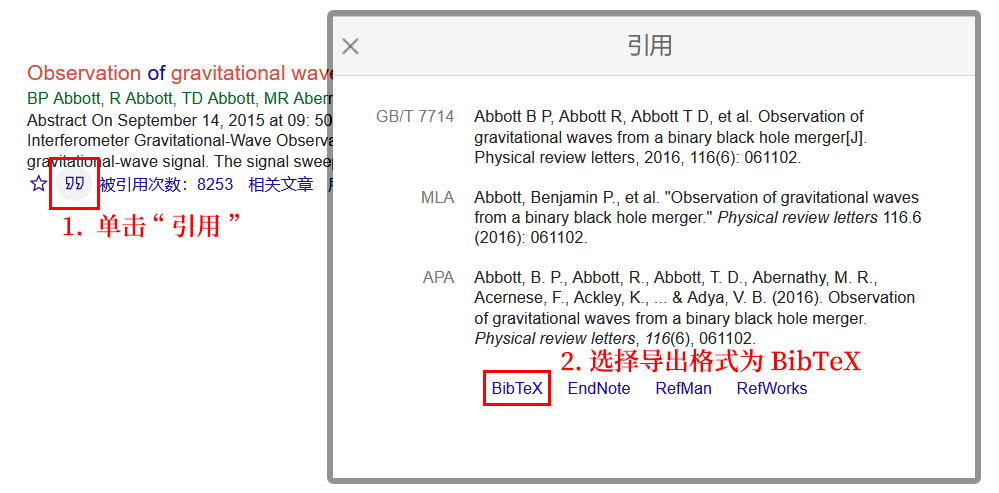
\includegraphics[width=10cm]{figure/AddBib.png}
                \label{fig:addbib}
            \end{figure}
        \item 在弹出框中,单击最下方 Bibtex 的链接;
        \item 在弹出的网页中复制所有代码至\textsf{thesisbib.bib},并根据需要做一些改动;
        \item 在您的论文中使用 \cmd{scite\{\}}引用相应的文献。
    \end{itemize}

    举个例子:在网页中将
    \begin{lstlisting}
@article{abbott2016observation,
    title={Observation of gravitational waves from a binary black hole merger},
    author={Abbott, Benjamin P and Abbott,% ...
    },
    journal={Physical review letters},
    volume={116},
    number={6},
    pages={061102},
    year={2016},
    publisher={APS}
}
    \end{lstlisting}
	复制进 \textsf{thesisbib.bib},在您的论文中使用
	\cmd{scite\{abbott2016observation\}}即可引用此文献。 
	再来一个\scite{ashirov2008tetramerization} ,
	网络上的资源引用\scite{buctthesis},等。

	另外,\emph{参考文献}格式控制文件\textsf{gbt7714-2005.bst}开源于
	\href{https://github.com/Haixing-Hu/GBT7714-2005-BibTeX-Style}{GitHub},
	其参考文献的著录可以用于参考。
    
    
\section{附录}\label{sec:app}
    在\textsf{buctthesis.tex}中以
    \begin{lstlisting}[firstnumber=68]
    \appendix
    \end{lstlisting}
    命令作为\emph{附录}部分的开始。与正文类似,只需往\textsf{chapter/app1.tex}等加入内容即可,
    除了编号使用大写字母之外都一样。见附录 \ref{app:1}。


\section{符号说明}\label{sec:deno}
	\emph{符号说明}部分的源文件位于\textsf{chapter/denotation.tex}。
    《规范》中未详细规定\emph{符号说明}的格式,这里附上一个以表格展示的代码:
    \begin{lstlisting}[caption=符号说明部分的跨页表格]
\begin{longtable}[c]{p{2.5cm}p{12cm}}
    \toprule
    \textbf{符号} & \textbf{说明} \\* \midrule
    \endfirsthead %
    \multicolumn{2}{r}{\bfseries (接上表)} \\
    \toprule
    \textbf{符号} & \textbf{说明} \\* \midrule
    \endhead %
    \bottomrule
    \endfoot
    \endlastfoot
        符号1   & 说明1     \\
        符号1   & 说明2     
    \\* \bottomrule
\end{longtable}        
    \end{lstlisting}

	本文档的\emph{符号说明}部分就是以此方式编辑,并展示了一个跨页表格的样式。
	详细代码请参见\textsf{denotation.tex}源代码和本手册\emph{符号说明}部分。


\section{致谢}
	\emph{致谢}部分的源文件位于\textsf{chapter/acknowledgement.tex},
	使用\texttt{acknowledgement}环境,往里面写入感谢的话就可以啦。
    \begin{lstlisting}
\begin{acknowledgement}
    % Words here.
    % ...
\end{acknowledgement}
    \end{lstlisting}


\section{其他}\label{sec:other}
    \subsection{脚注}
	本模板采用带圈数字脚注,计数跨章重置,使用命令 \cmd{footnote}。
	前方高能\footnote{我是可爱的脚注}。

	有些情况下(比如在表格环境、各种盒子内)使用 \cmd{footnote}并不能正确生成脚注。
	我们可以分两步进行,先使用 \cmd{footnotemark} 为脚注计数,
	再在合适的位置用 \cmd{footnotetext} 生成脚注。比如:
    \begin{table}[H]
        \centering
        \begin{tabular}{ll}
        \hline
            人之初,性本善 & 性相近,习相远。\\
            苟 \footnotemark 不教,性乃迁 & 教之道,贵以专。\\
        \hline
    \end{tabular}
    \end{table}
    \footnotetext{苟:如果}

    \subsection{列表环境}\label{subsec:items}
	本模板提供了三种列表环境:不编号的\texttt{itemize}、编号的\texttt{enumerate}
	和使用关键字的\texttt{description}环境。在文档的中英文\emph{摘要}部分分别展示了
	最基础的编号和不编号的列表环境;上面三种列表环境可以嵌套使用(至多四层),
	且会自动处理不同层次的缩进和编号,如下所示:
    \begin{itemize}
        \item 一条
        \item 次条
        \item 这一条可以分为\dots
            \begin{itemize}
            \item 子一条
            \end{itemize}
        \end{itemize}
    稍复杂一点的,如:
        \begin{enumerate}
            \item 中文
            \begin{description}
                \item[文言文] 古代汉语
                \item[白话文] 现代汉语
                \begin{enumerate}
                    \item 口语
                        \begin{enumerate}
                            \item 普通话
                            \item 方言
                        \end{enumerate}
                    \item 书面语
                    \end{enumerate}
            \end{description}
            \item English
        \end{enumerate}

    \subsection{\textsf{hyperref}宏包的设置}
	这里不是论文要求所必须的,但是为了方便使用和查看还是做了部分设置,
	其位于宏包文件\textsf{buctthesis.sty}的最后部分:
    \begin{lstlisting}[firstnumber=428]
\hypersetup{
    colorlinks=true,           % 使用彩色文字链接(禁用链接外的方框)
    %hidelinks,                % 隐藏链接颜色
    bookmarksnumbered=true,    % 书签中,章节编号
    pdfhighlight=/N,           % 点击链接时的外观
    breaklinks=true,           % 允许断行
}
    \end{lstlisting}
	为了便于查看,模板默认打开超链接的颜色;否则请将\texttt{hidelinks}命令取消注释,
	这会将所有超链接设置为黑色。